\documentclass[a4paper,11pt]{article}

\usepackage{array}
% \usepackage{fullpage}
% \usepackage{html}
\usepackage{graphicx}
\usepackage[pdfborder={0 0 1},colorlinks]{hyperref}
\usepackage[titletoc]{appendix}
\usepackage[section=section,acronym,toc,style=list]{glossaries}

\newcommand{\amu}{\textit{amu}}
\newcommand{\nm}{\textit{nm}}
\newcommand{\nmsquare}{$nm^2$}
\newcommand{\vacfunits}{$nm^2s^{-2}$}
\newcommand{\ps}{\textit{ps}}
\newcommand{\invnm}{$nm^{-1}$}
\newcommand{\ns}{\textit{ns}}
\newcommand{\thz}{\textit{THz}}
\newcommand{\qval}{\textit{q}}
\newcommand{\qvect}{\textit{q}-vector}
\newcommand{\qvects}{\textit{q}-vectors}
\newcommand{\qshell}{\textit{q}-shell}
\newcommand{\qshells}{\textit{q}-shells}

\makeglossaries
\newacronym{CN}{\textit{CN}}{\textbf{C}oordination \textbf{N}umber}
\newacronym{COMT}{\textit{COMT}}{\textbf{C}enter \textbf{O}f \textbf{M}ass \textbf{T}rajectory}
\newacronym{DOS}{\textit{DOS}}{\textbf{D}ensity \textbf{O}f \textbf{S}tates}
\newacronym{FCA}{\textit{FCA}}{\textbf{F}ast \textbf{C}orrelation \textbf{A}lgorithm}
\newacronym{FFT}{\textit{FFT}}{\textbf{F}ast \textbf{F}ourier \textbf{T}ransform}
\newacronym{EISF}{\textit{EISF}}{\textbf{E}lastic \textbf{I}ncoherent \textbf{S}tructure \textbf{F}actor}
\newacronym{GMFT}{\textit{GMFT}}{\textbf{G}lobal \textbf{M}otion \textbf{F}iltered \textbf{T}rajectory}
\newacronym{MD}{\textit{MD}}{\textbf{M}olecular \textbf{D}ynamics}
\newacronym{MDANSE}{\textit{MDANSE}}{\textbf{M}olecular \textbf{D}ynamics \textbf{Analysis} for \textbf{N}eutron \textbf{S}cattering \textbf{E}xperiments}
\newacronym{MSD}{\textit{MSD}}{\textbf{M}ean-\textbf{S}quare \textbf{D}isplacement}
\newacronym{PDF}{\textit{PDF}}{\textbf{P}air \textbf{D}istribution \textbf{F}unction}
\newacronym{RBT}{\textit{RBT}}{\textbf{R}igid-\textbf{B}ody \textbf{T}rajectory}
\newacronym{RDF}{\textit{RDF}}{\textbf{R}adial \textbf{D}istribution \textbf{F}unction}
\newacronym{ROG}{\textit{ROG}}{\textbf{R}adius \textbf{O}f \textbf{G}yration}
\newacronym{RMSD}{\textit{RMSD}}{\textbf{R}oot \textbf{M}ean-\textbf{S}quare \textbf{D}eviation}
\newacronym{SD}{\textit{SD}}{\textbf{S}patial \textbf{D}ensity}
\newacronym{TCF}{\textit{TCF}}{\textbf{T}otal \textbf{C}orrelation \textbf{F}unction}
\newacronym{VACF}{\textit{VACF}}{\textbf{V}elocity \textbf{A}uto\textbf{C}orrelation \textbf{F}unction}
\glsaddall

\begin{document}

\begin{titlepage}

\begin{center}

\vspace{2cm}
 
\hrule height 0.1cm
\vspace{0.5cm}
{\Huge \bfseries MDANSE - theoretical background}\\
\vspace{0.5cm}
\hrule height 0.1cm

\vspace{1.0cm}
 
{\large \today}\\

\vspace{1.0cm}

{\large \textbf{Description}}\\

\end{center}

\noindent This note describes the theoretical background of the analyses in \textit{MDANSE}. \textit{MDANSE} (\textbf{M}olecular \textbf{D}ynamics \textbf{A}nalysis 
for \textbf{N}eutron \textbf{S}cattering \textbf{E}xperiments) is a python application for analyzing molecular dynamics simulation data.

%\footnote{$^{a}$Institut Laue-Langevin 6, rue Jules Horowitz BP 156 - 38042 Grenoble Cedex 9, France}

\end{titlepage}

\tableofcontents{}

\newpage

\section{Dynamics Analyses}
\label{dynamics_menu}
The following analyses are described:
\begin{itemize}
\item Mean-Square Displacement
\item Root Mean-Square Displacement
\item Radius Of Gyration
\item Velocity AutoCorrelation Function
\item Density Of States
\item Global Motion Trajectory
\item Center Of Mass Trajectory
\item Rigid-Body Trajectory
\item Center Of Mass Trajectory
\end{itemize}

\subsection{Mean-Square Displacement}
\label{msd}
\paragraph{Theory and implementation\\}
\label{msd_theory}
Molecules in liquids and gases do not stay in the same place, but move constantly. 
This process is called diffusion and it happens quite naturally in fluids at equilibrium. 
During this process, the motion of an individual molecule does not follow a simple path \cite{Democritus}. 
As it travels, the molecule undergoes some collisions with other molecules which prevent 
it from following a straight line. If the path is examined in close detail, it will be seen 
to be a good approximation to a random walk. Mathematically, a random walk is a series of steps 
where each step is taken in a completely random direction from the one before. 
This kind of path was famously analysed by Albert Einstein in a study of Brownian motion. He showed 
that the \gls{MSD}\ of a particle following a random walk is 
proportional to the time elapsed. This relationship can be written as
\begin{equation}
<r^2> = 6Dt + C
\end{equation}
where $<r^2>$ is the \gls{MSD}\ and \textit{t} is the time. \textit{D} and \textit{C} are constants. 
The constant \textit{D} defines the so-called diffusion coefficient.

The figure \ref{fig:msd_water} shows an example of a \gls{MSD}\ analysis performed on a waterbox of 768 water molecules.
\begin{figure}[h!]
\begin{center}
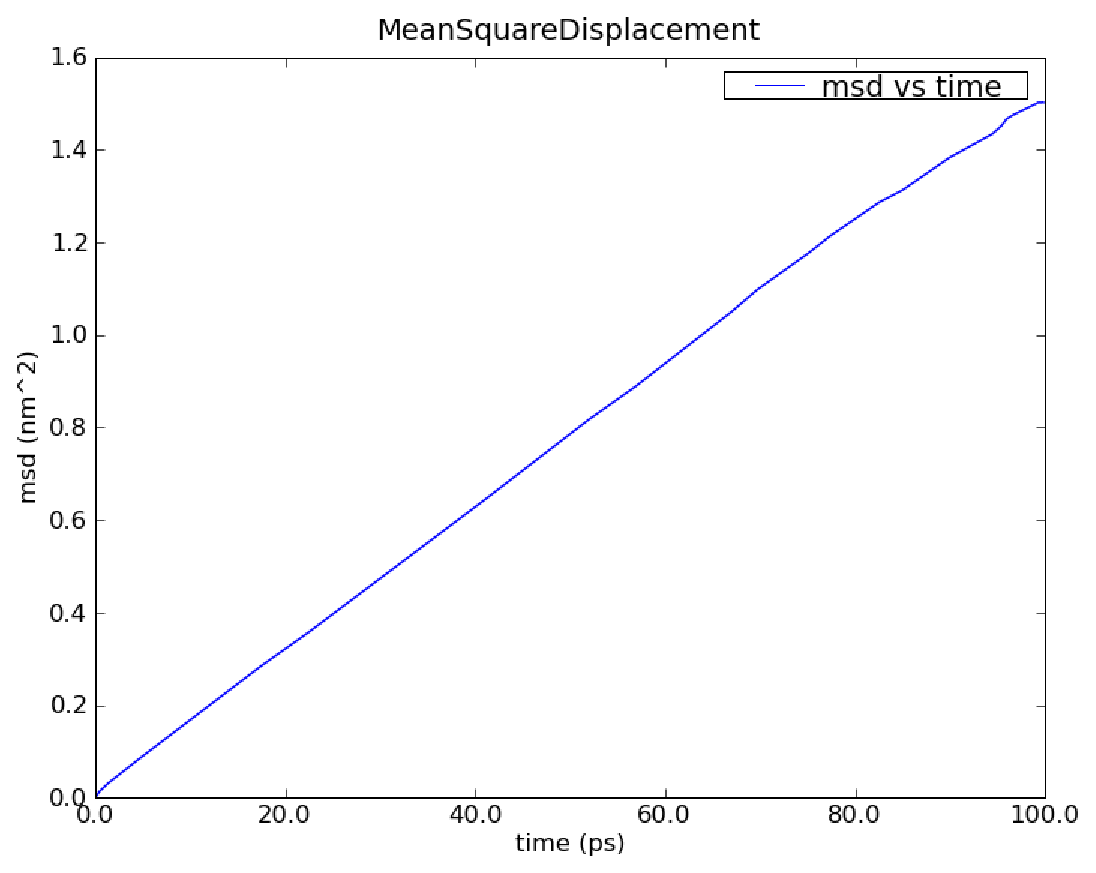
\includegraphics[width=10cm]{figures/msd_water.eps}
\end{center}
\caption[Examples of calculated \textit{MSD} with \textit{MDANSE}]{\gls{MSD} calculated for a 100 ps MD simulation of 256 water molecules using NPT condition at 1 bar and 300 K.}
\label{fig:msd_water}
\end{figure}

To get the diffusion coefficient out of this plot, the slope of the linear part of the plot should be calculated.

Defining,
\begin{equation}
\textbf{d}_{\alpha}(t,t_0) \doteq \textbf{R}_\alpha(t_0 + t) - \textbf{R}_\alpha(t_0).
\end{equation}
the \gls{MSD}\ of particle $\alpha$ can be defined as:
\begin{equation}
\label{eq:msd}
\Delta^2_\alpha(t) = \left\langle \textbf{d}^2_\alpha(t,t_0) \right\rangle_{t_0}
\end{equation}
where $\textbf{R}_\alpha(t_0)$ and $\textbf{R}_\alpha(t_0 + t)$ are respectively the position of particle $\alpha$ at 
times $t_0$ and $t_0+t$.
One can introduce a \gls{MSD}\ with respect to a given axis \textbf{n}:
\begin{equation}
\label{eq:msd_n}
\Delta^2_\alpha(t,t_0;\textbf{n}) \doteq \left\langle
d^2_\alpha(t,\tau;\textbf{n})\right\rangle_{t_0}
\end{equation}
with
\begin{equation}
d_{\alpha}(t,t_0;\textbf{n}) \doteq \textbf{n}\cdot \textbf{d}_{\alpha}(t,t_0).
\end{equation}
The calculation of \gls{MSD}\ is the standard way
to obtain diffusion coefficients from \gls{MD} simulations. Assuming
Einstein-diffusion in the long time limit one has for isotropic
systems
\begin{equation}
\label{eq:diffusion_coeff}
D_\alpha = \lim_{t\to\infty} \frac{1}{6t} \Delta^2_\alpha(t).
\end{equation}

There exists also a well-known relation between the \gls{MSD}\ and the velocity 
autocorrelation function. Writing $\textbf{d}_\alpha(t) = \int_{0}^{t}d\tau\,\textbf{v}_\alpha(\tau)$  in Eq.
(\ref{eq:msd}) one can show (see e.g. \cite{Yip:1980}) that 
\begin{equation}
\label{eq:msd_vacf}
\Delta^2_\alpha(t) = 6 \int_{0}^{t}d\tau\,(t - \tau)
C_{vv ; \alpha\alpha}(\tau).
\end{equation}
Using now the definition (\ref{eq:diffusion_coeff}) of the diffusion coefficient one
obtains the relation
\begin{equation}
\label{eq:d_vacf}
D_\alpha = \int_{0}^{t}d\tau\, C_{vv ; \alpha\alpha}(\tau).
\end{equation}
With Eq. (\ref{eq:dos_alpha}) this can  also be written as
\begin{equation}
\label{eq:d_dos}
D_\alpha = \pi \tilde C_{vv ; \alpha\alpha}(0).
\end{equation}

Computationally, the \gls{MSD}\ is calculated using the \gls{FCA} \cite{Kneller:KFA}. In this 
framework, in the discrete case, the mean-square displacement of a particle is given by
\begin{equation}
\label{eq:msd_discrete}
\Delta^2(m) = \frac{1}{N_t - m}\sum_{k=0}^{N_t-m-1}
[\textbf{r}(k+m) - \textbf{r}(k)]^2, \qquad m = 0\ldots N_t-1,
\end{equation}
where $\textbf{r}(k)$ is the particle trajectory and $N_t$ is the the number of frames of the trajectory. We define now the
auxiliary function
\begin{equation}
S(m) \doteq \sum_{k=0}^{N_t-m-1}[\textbf{r}(k+m) - \textbf{r}(k)]^2, 
\qquad m = 0\ldots N_t-1,
\end{equation}
which is splitted as follow:
\begin{eqnarray}
S(m)          &= &S_{AA+BB}(m) - 2 S_{AB}(m),\\
S_{AA+BB}(m)  &= &\sum_{k=0}^{N_t-m-1}[\textbf{r}^2(k+m) + \textbf{r}^2(k)], \\
S_{AB}(m)     &= &\sum_{k=0}^{N_t-m-1} \textbf{r}(k)\cdot\textbf{r}(k+m). 
\end{eqnarray}
The function $S_{AB}(m)$ can be computed using the \gls{FCA} method described
in Section \ref{fca}. For $S_{AA+BB}(m)$ the following recursion
relation holds:
\begin{eqnarray}
S_{AA+BB}(m) &= &S_{AA+BB}(m-1) - \textbf{r}^2(m-1)  - \textbf{r}^2(N_t - m),\\
S_{AA+BB}(0) &= &\sum_{k=0}^{N_t-1} \textbf{r}^2(k).
\end{eqnarray}
This allows one to construct the following efficient scheme for the
computation of the \gls{MSD}:
\begin{enumerate}
\item Compute $DSQ(k) = \textbf{r}^2(k),\qquad k = 0\ldots N_t-1;\qquad
      DSQ(-1) = DSQ(N_t) = 0$.
\item Compute $SUMSQ = 2\cdot\sum_{k=0}^{N_t-1} DSQ(k)$.
\item Compute $S_{AB}(m)$ using the \gls{FFT} method.
\item Compute \textit{MSD(m)} in the following loop:
      \begin{displaymath}
      \begin{array}{ll}
                &\begin{array}{ll}
                 SUMSQ  &\leftarrow SUMSQ - DSQ(m-1) - DSQ(N_t - m)\\
                 MSD(m) &\leftarrow (SUMSQ - 2\cdot S_{AB}(m)/(N_t-m)\\
                \end{array}\\
                 &m\; \mbox{running from}\; 0 \;\mbox{to}\; N_t - 1\\
      \end{array}
      \end{displaymath}
\end{enumerate}
It should be noted that the efficiency of this algorithm is the same
as for the \gls{FCA} computation of time correlation functions since the
number of operations in step (1), (2), and (4) grows linearly with
$N_t$.

\subsection{Root Mean-Square Deviation}
\label{rmsd}
\paragraph{Theory and implementation\\}
\label{rmsd_theory}
The \gls{RMSD} is maybe the most popular estimator of structural similarity. It is a 
numerical measure of the difference between two structures that can be defined as:
\begin{equation}
\label{eq:rmsd}
RMSD(t) = \sqrt{\frac{\sum_{\alpha = 1}^{N_{\alpha}}({\bf r}_{\alpha}(t) - {\bf r}_{\alpha}(t_{ref}))}{N_{\alpha}}}
\end{equation}
where $N_{\alpha}$ is the number of atoms of the system, and ${\bf r}_{\alpha}(t)$ and ${\bf r}_{\alpha}(t_{ref})$ are 
respectively the position of atom $\alpha$ at time $t$ and $t_{ref}$ where $t_{ref}$ is a reference time usually 
choosen as the first step of the simulation.
Typically, \gls{RMSD} is used to quantify the structural evolution of the system during the simulation. It can 
provide precious information about the system especially if it reached equilibrium or conversely if major
structural changes occured during the simulation.

In \gls{MDANSE}, \gls{RMSD} is computed using the discretized version of equation \ref{eq:rmsd}:
\begin{equation}
\label{eq:rmsd_num}
RMSD(n\cdot\Delta t) = \sqrt{\frac{\sum_{\alpha = 1}^{N_{\alpha}}({\bf r}_{\alpha}(t) - {\bf r}_{ref}(t))}{N_{\alpha}}},
\qquad n = 0\ldots N_t - 1.
\end{equation}
where $N_t$ is the number of frames and $\Delta t$ is the time step.

\subsection{Radius of gyration}
\label{rog}
\paragraph{Theory and implementation\\}
\label{rog_theory}
\gls{ROG} is the name of several related measures of the size of an object, a surface, or an ensemble of 
points. It is calculated as the Root Mean Square Distance between the system and a reference that can be either 
the center of gravity of the system either a given axis. In \gls{MDANSE}, the reference is choosen to be the center 
of gravity of the system under study. Mathematically, it can be defined as:
\begin{equation}
\label{eq:rog}
ROG(t) = \sqrt{\frac{\sum_{\alpha = 1}^{N_{\alpha}}({\bf r}_{\alpha}(t) - {\bf r}_{cms}(t))}{N_{\alpha}}}
\end{equation}
where $N_{\alpha}$ is the number of atoms of the system, and ${\bf r}_{\alpha}(t)$ and ${\bf r}_{cms}(t)$ are 
respectively the position of atom $\alpha$ and the center of mass of the system at time $t$.

\gls{ROG} describes the overall spread of the molecule and as such is a good measure for the molecule compactness. For
example, it can be useful when monitoring folding process.

In \gls{MDANSE}, \gls{ROG} is computed using the discretized version of equation \ref{eq:rog}:
\begin{equation}
\label{eq:rog_num}
ROG(n\cdot\Delta t) = \sqrt{\frac{\sum_{\alpha = 1}^{N_{\alpha}}({\bf r}_{\alpha}(t) - {\bf r}_{cms}(t))}{N_{\alpha}}},
\qquad n = 0\ldots N_t - 1.
\end{equation}
where $N_t$ is the number of frames and $\Delta t$ is the time step.

\subsection{Angular Correlation}
\label{ac}
\paragraph{Theory and implementation\\}
\label{ac_theory}
The angular correlation analysis computes the autocorrelation of a set of vectors describing the extent of a molecule in three 
orthogonal directions. This kind of analysis can be useful when trying to highlight the fact that a molecule is constrainted 
in a given direction.

For a given triplet of non-colinear atoms \textit{g}=(\textbf{a1},\textbf{a2},\textbf{a3}), one can derive an orthonormal 
set of three vectors ${\bf v}_1$, ${\bf v}_2$, ${\bf v}_3$ using the following scheme:

\begin{itemize}
\item ${\bf v}_1 = \frac{{\bf n}_{1} + {\bf n}_{2}}{||{\bf n}_{1} + {\bf n}_{2}||}$
where ${\bf n}_{1}$ and ${\bf n}_{2}$ are respectively the normalized vectors along (\textbf{a1},\textbf{a2}) 
and (\textbf{a1},\textbf{a3}) directions.
\item ${\bf v}_2$ is defined as the clockwise normal vector orthogonal to ${\bf v}_1$ that belongs to the plane 
defined by \textbf{a1}, \textbf{a2} and \textbf{a3} atoms
\item $\vec{v_3} = \vec{v_1} \times \vec{v_2}$
\end{itemize}

Thus, one can define the following autocorrelation functions for the vectors ${\bf v}_1$, ${\bf v}_2$ and ${\bf v}_3$ 
defined on triplet \textit{t}:
\begin{equation}
\label{eq:ac_per_triplet}
AC_{g,i} (t) = \langle {\bf v}_{t,i}(0)\cdot{\bf v}_{t,i}(t)\rangle, \qquad  i = 1,2,3
\end{equation}

And the angular correlation averaged over all triplets is:
\begin{equation}
\label{eq:ac}
AC_i(t) = \sum_{g=1}^{N_{triplets}} AC_{g,i}(t), \qquad  i = 1,2,3
\end{equation}
where $N_{triplets}$ is the number of selected triplets.

\subsection{Velocity Autocorrelation Function}
\label{vacf}
\paragraph{Theory and implementation\\}
\label{vacf_theory}
The \gls{VACF} is another interesting property describing the dynamics of a 
molecular system. Indeed, it reveals the underlying nature of the forces acting on the system. 

In a molecular system that would be made of non interacting particles, the velocities would be constant at 
any time triggering the \gls{VACF} to be a constant value. Now, if we think about a system with small interactions such as in a
gas-phase, the magnitude and direction of the velocity of a particle will change gradually over time due to its 
collision with the other particles of the molecular system. In such a system, the \gls{VACF} will be represented by a
decaying exponential.

In the case of solid phase, the interaction are much stronger and, as a results, the atoms are bound to a given 
position from which they will move backwards and forwards oscillating between positive and negative values of 
their velocity. The oscillations will not be of equal magnitude however, but will decay in time, because there 
are still perturbative forces acting on the atoms to disrupt the perfection of their oscillatory motion. So, in 
that case the \gls{VACF} will look like a damped harmonic motion.

Finally, in the case of liquid phase, the atoms have more freedom than in solid phase and because of the diffusion 
process, the oscillatory motion seen in solid phase will be cancelled quite rapidly depending on the density of the
system. So, the \gls{VACF} will just have one very damped oscillation before decaying to zero. This decaying time can be
considered as the average time for a collision between two atoms to occur before they diffuse away.

Mathematically, the \gls{VACF} of atom $\alpha$ in an atomic or molecular system is usually defined as
\begin{equation}
\label{eq:vacf}
C_{vv ; \alpha\alpha}(t) \doteq
\frac{1}{3}\langle {\bf v}_\alpha(t_0)\cdot{\bf v}_\alpha(t_0+t)\rangle_{t_0}.
\end{equation}
In some cases, e.g. for non-isotropic systems, it is useful to define \gls{VACF} along a given axis,
\begin{equation}
\label{eq:vacf_n}
C_{vv ; \alpha\alpha}(t;{\bf n}) \doteq
\langle v_\alpha(t_0;{\bf n})v_\alpha(t_0+t;{\bf n})\rangle_{t_0},
\end{equation}
where $v_\alpha(t;{\bf n})$ is given by
\begin{equation}
v_\alpha(t;{\bf n}) \doteq 
{\bf n}\cdot{\bf v}_{\alpha}(t).
\end{equation}
The vector \textit{\textbf{n}} is a unit vector defining a space-fixed axis.

The \gls{VACF} of the particles in a many body system can be related to the
incoherent dynamic structure factor by the relation:
\begin{equation}
\label{eq:sqw_dos}
lim_{q\to 0} \frac{\omega^2}{q^2}{\cal S}({\bf q},\omega) =
G(\omega), 
\end{equation}
where $G(\omega)$ is the \gls{DOS}. For an isotropic system it reads
\begin{eqnarray}
\label{eq:dos}
G(\omega) &= &\sum_{\alpha}b^2_{\alpha,inc}
\tilde C_{vv ; \alpha\alpha}(\omega),\\
\label{eq:dos_alpha}
\tilde C_{vv ; \alpha\alpha}(\omega) &= &
\frac{1}{2\pi}\int_{-\infty}^{+\infty}dt\, \exp[-i\omega t] 
C_{vv ; \alpha\alpha}(t).
\end{eqnarray}
For non-isotropic systems relation (\ref{eq:sqw_dos}) holds if the \gls{DOS} is computed from the atomic velocity 
autocorrelation functions $C_{vv ; \alpha\alpha}(t;{\bf n}_q)$, where ${\bf n}_q$ is the unit vector in the 
direction of \textit{\textbf{q}}.

\subsection{Density Of States}
\label{dos}
\paragraph{Theory and implementation\\}
\label{dos_theory}
\gls{MDANSE} calculates the power spectrum of the \gls{VACF}, which in case of the mass-weighted \gls{VACF} defines the phonon 
discrete \gls{DOS}, (see Section \ref{vacf_theory}) defined as:
\begin{eqnarray}
DOS(n\cdot\Delta \nu)  &\doteq &\sum_{\alpha} \omega_\alpha 
\tilde C_{vv ; \alpha\alpha}(n\cdot\Delta \nu),\qquad n = 0\ldots N_t - 1.
\end{eqnarray}
$N_t$ is the total number of time steps and $\Delta\nu = 1/(2N_t \Delta t)$ is the frequency step. $DOS(n\cdot\Delta\nu)$ can 
be computed either for the isotropic case or with respect to a user-defined axis. The spectrum $DOS(n\cdot\Delta \nu)$ is computed from the 
\textit{unnormalized} \gls{VACF}, such that \textit{DOS(0)} gives an approximate value for the diffusion constant 
$D = \sum_\alpha D_\alpha$ (see Eqs. \ref{eq:d_vacf} and \ref{eq:d_dos}). $DOS(n\cdot\Delta \nu)$ is smoothed by 
applying a Gaussian window in the time domain \cite{Harris} (see Section \ref{fca}). Its width in the time domain is 
$\sigma_t=\alpha/T$, where $T$ is the length of 
the simulation. We remark that the diffusion constant obtained from \gls{DOS} is biased due to the spectral smoothing procedure since 
the \gls{VACF} is weighted by this window Gaussian function. \gls{MDANSE} computes the density of states starting from both atomic velocities 
and atomic coordinates. In this case the velocities are computed by numerical differentiation of the coordinate trajectories correcting 
first for possible jumps due to periodic boundary conditions.

\subsection{Global Motion Filtered Trajectory}
\label{gmft}
\paragraph{Theory and implementation\\}
\label{gmft_theory}
It is often of interest to separate global motion from internal motion, both for quantitative analysis 
and for visualization by animated display. Obviously, this can be done under the hypothesis that global and internal 
motions are decoupled within the length and timescales of the analysis. \gls{MDANSE} can create \gls{GMFT} by filtering out global 
motions (made of the three translational and rotational degrees of freedom), either on the whole system or on an user-defined subset, 
by fitting it to a reference structure (usually the first frame of the \gls{MD}). Global motion filtering uses a straightforward 
algorithm:
\begin{itemize}
\item for the first frame, find the linear transformation such that the coordinate origin becomes the center of mass of 
the system and its principal axes of inertia are parallel to the three coordinates axes (also called principal axes 
transformation),
\item this provides a reference configuration ${\cal C}_{ref}$,
\item for any other frames \textit{f}, finds and applies the linear transformation that minimizes the RMS distance between 
frame \textit{f} and ${\cal C}_{ref}$.
\end{itemize} 
The result is stored in a new trajectory file that contains only internal motions. This analysis can be useful in case where diffusive 
motions are not of interest or simply not accessible to the experiment (time resolution, powder analysis \ldots).


\subsection{Rigid-Body Trajectory}
\label{rbt}
\paragraph{Theory and implementation\\}
\label{rbt_theory}
To analyze the dynamics of complex molecular systems it is often desirable to consider the overall motion of 
molecules or molecular subunits. We will call this motion rigid-body motion in the following. Rigid-body motions 
are fully determined by the dynamics of the centroid, which may be the center-of-mass, and the dynamics of the
angular coordinates describing the orientation of the rigid body. The angular coordinates are the appropriate 
variables to compute angular correlation functions of molecular systems in space and time. In most cases, however, 
these variables are not directly available from \gls{MD}\ simulations since \gls{MD}\ algorithms typically work in cartesian coordinates. 
Molecules are either treated as flexible, or, if they are treated as rigid, constraints are taken into account in the 
framework of cartesian coordinates \cite{Berendsen}. In \gls{MDANSE}, \gls{RBT} can be defined from a 
\gls{MD} trajectory by fitting rigid reference structures, defining a (sub)molecule, to the corresponding structure in each time 
frame of the trajectory. Here `fit' means the optimal superposition of the structures in a least-squares sense. We will 
describe now how rigid body motions, i.e. global translations and rotations of molecules or  subunits of complex molecules, 
can be extracted from a \gls{MD} trajectory. A more detailed presentation is given in \cite{Kneller:1991}. We define 
an optimal rigid-body trajectory in the following way: for each time frame of the trajectory the atomic positions of a rigid 
reference structure, defined by the three cartesian components of its centroid (e.g. the center of mass) and three angles, are as 
close as possible to the atomic positions of the corresponding structure in  the \gls{MD} configuration. Here `as close as possible' means as close 
as possible in a least-squares sense.  

\subparagraph{Optimal superposition.} We consider a given time frame in which the atomic positions of a (sub)molecule are 
given by  ${\bf x}_\alpha,\,\alpha = 1\ldots N$. The corresponding positions in the reference structure are denoted as 
${\bf x}^{(0)}_\alpha,\,\alpha = 1\ldots N$. For both the given structure and the reference structure we introduce the yet 
undetermined centroids ${\bf X}$ and  ${\bf X}^{(0)}$, respectively, and define the deviation 
\begin{equation}
\label{eq:delta}
{\bf \Delta}_\alpha \doteq
{\bf D}({\bf q})\left[{\bf x}^{(0)}_\alpha - {\bf X}^{(0)}\right] -   
       \left[{\bf x}_\alpha - {\bf X}\right].   
\end{equation} 
Here ${\bf D}({\bf q})$ is a rotation matrix which depends on also yet undetermined angular coordinates which we chose to 
be {\em quaternion parameters}, abbreviated as vector ${\bf q} = (q_0,q_1,q_2,q_3)$. The quaternion parameters fulfill the 
normalization condition ${\bf q}\cdot{\bf q} = 1$ \cite{Altmann}. The target function to be minimized is now defined as
\begin{equation}
m({\bf q};{\bf X},{\bf X}^{(0)}) = 
\sum_\alpha \omega_\alpha |{\bf\Delta}|^2_\alpha.
\end{equation}
where $\omega_\alpha$ are atomic weights (see Section \ref{weighting_scheme}). The minimization with respect to the centroids 
is decoupled from the minimization with respect to the quaternion parameters and yields
\begin{eqnarray}
{\bf X}       &= &\sum_\alpha \omega_\alpha\,{\bf x}_\alpha,\\
{\bf X}^{(0)} &= &\sum_\alpha \omega_\alpha\,{\bf x}^{(0)}_\alpha.
\end{eqnarray} 
We are now left with a minimization problem for the rotational part which can be written as
\begin{equation}
\label{eq:minimize_rot}
m({\bf q}) = \sum_\alpha \omega_\alpha 
\left[{\bf D}({\bf q}){\bf r}^{(0)}_\alpha - {\bf r}_\alpha\right]^2
\stackrel{!}{=} Min.
\end{equation}
The relative position vectors
\begin{eqnarray}
{\bf r}_\alpha        &= &{\bf x}_\alpha - {\bf X},\\
{\bf r}^{(0)}_\alpha  &= &{\bf x}^{(0)}_\alpha - {\bf X}^{(0)},
\end{eqnarray} 
are fixed and the rotation matrix reads \cite{Altmann}
\begin{equation}
\label{eq:d_quat}
{\bf D}({\bf q}) = 
\left(
\begin{array}{ccc}
 q_0^2+q_1^2-q^2_2-q^2_3  &2(-q_0q_3+q_1q_2) &2(q_0q_2+q_1q_3) \\
 2(q_0q_3+q_1q_2)  &q_0^2+q_2^2-q^2_1-q^2_3  &2(-q_0q_1+q_2q_3)\\
 2(-q_0q_2+q_1q_3) &2(q_0q_1+q_2q_3)  &q_0^2+q_3^2-q^2_1-q^2_2  
\end{array}
\right).
\end{equation}

\subparagraph{Quaternions and rotations.} The rotational minimization problem can be elegantly solved by using quaternion algebra.
Quaternions are so-called hypercomplex numbers, having a real unit, ${\bf 1}$, and three imaginary units, 
${\bf I}$, ${\bf J}$, and ${\bf K}$. Since ${\bf I}{\bf J} = {\bf K}$ (cyclic), quaternion multiplication is not commutative. 
A possible matrix representation of an arbitrary quaternion,
\begin{equation}
{\bf A} = a_0\cdot{\bf 1} + a_1\cdot{\bf I} + a_2\cdot{\bf J} + 
          a_3\cdot{\bf K},
\end{equation}
reads 
\begin{equation}
\label{eq:a_mat}
 {\bf A} = \left( \begin{array}{rrrr}
                  a_0 &-a_1 &-a_2 &-a_3 \\
                  a_1 & a_0 &-a_3 & a_2 \\
                  a_2 & a_3 & a_0 &-a_1 \\
                  a_3 &-a_2 & a_1 & a_0
                  \end{array} 
           \right).
\end{equation}
The components $a_\nu$ are real numbers. Similarly as normal complex numbers allow one to represent rotations in a plane, quaternions 
allow one to represent rotations in space. Consider the quaternion representation of a vector ${\bf r}$, which is given by 
\begin{equation}
{\bf R} = x\cdot{\bf I} + y\cdot{\bf J} + z\cdot{\bf K},
\end{equation}  
and perform the operation
\begin{equation}
{\bf R}' = {\bf Q}{\bf R}{\bf Q}^T,
\end{equation}  
where ${\bf Q}$ is a normalized quaternion,
\begin{equation}
\|{\bf Q}\|^2 \doteq
q_0^2 + q_1^2 + q_2^2 + q_3^2 = \frac{1}{4}tr\{{\bf Q}^T{\bf Q}\} = 1. 
\end{equation}
The symbol $tr$ stands for `trace'. We note that a normalized quaternion is represented by an {\em orthogonal} $4\times 4$ 
matrix. ${\bf R}'$ may then be written  as
\begin{equation}
{\bf R}' = x'\cdot{\bf I} + y'\cdot{\bf J} + z'\cdot{\bf K},
\end{equation}
where the components $x',y',z'$, abbreviated as ${\bf r}'$, are given by
\begin{equation}
{\bf r}' = {\bf D}({\bf q}){\bf r}.
\end{equation}
The matrix ${\bf D}({\bf q})$ is the rotation matrix defined in
(\ref{eq:d_quat}).

\subparagraph{Solution of the minimization problem.} In quaternion algebra, the rotational minimization problem may now be 
phrased as follows:
\begin{equation}
\label{eq:minimize_rot_quat_1}
m({\bf q}) = \sum_\alpha \omega_\alpha 
\|{\bf Q}{\bf R}^{(0)}_\alpha{\bf Q}^T - {\bf R}_\alpha\|^2
\stackrel{!}{=} Min.
\end{equation}
Since the matrix ${\bf Q}$ representing a normalized quaternion is orthogonal this may also be written as
\begin{equation}
\label{eq:minimize_rot_quat_2}
m({\bf q}) = \sum_\alpha \omega_\alpha 
\|{\bf Q}{\bf R}^{(0)}_\alpha - {\bf R}_\alpha{\bf Q}\|^2.
\stackrel{!}{=} Min.
\end{equation}
This follows from the simple fact that  $\|{\bf A}\| = \|{\bf A}{\bf Q}\|$, if ${\bf Q}$ is normalized. 
Eq. (\ref{eq:minimize_rot_quat_2}) shows that the target function to be minimized can be written as a simple quadratic 
form in the quaternion parameters \cite{Kneller:1991}, \begin{eqnarray}
\label{eq:quad_form}
m({\bf q}) &= &{\bf q}\cdot{\bf M}{\bf q},\\
{\bf M} &= &\sum_\alpha \omega_\alpha {\bf M}_\alpha.
\end{eqnarray}
The matrices ${\bf M}_\alpha$ are positive semi-definite matrices depending on the positions ${\bf r}_\alpha$ and 
${\bf r}^{(0)}_\alpha$:
\begin{equation}
\left.
\begin{array}{lll}
M_{\alpha,11} &= &
  x_\alpha^2 + y_\alpha^2 + z_\alpha^2 
+ x_{0\alpha}^2 + y_{0\alpha}^2 + z_{0\alpha}^2   
-2x_\alpha x_{0\alpha} -2y_\alpha y_{0\alpha} -2z_\alpha z_{0\alpha}
\\
M_{\alpha,12} &= &2(y_\alpha z_{0\alpha} - z_\alpha y_{0\alpha})\\
M_{\alpha,13} &= &2(-x_\alpha z_{0\alpha} + z_\alpha x_{0\alpha})\\
M_{\alpha,14} &= &2(x_\alpha y_{0\alpha} - y_\alpha x_{0\alpha})\\
M_{\alpha,22} &= &
  x_\alpha^2 + y_\alpha^2 + z_\alpha^2 
+ x_{0\alpha}^2 + y_{0\alpha}^2 + z_{0\alpha}^2   
-2x_\alpha x_{0\alpha} +2y_\alpha y_{0\alpha} +2z_\alpha z_{0\alpha}
\\
M_{\alpha,23} &= &-2(x_\alpha y_{0\alpha} + y_\alpha x_{0\alpha})\\
M_{\alpha,24} &= &-2(x_\alpha z_{0\alpha} + z_\alpha x_{0\alpha})\\
M_{\alpha,33} &= &
  x_\alpha^2 + y_\alpha^2 + z_\alpha^2 
+ x_{0\alpha}^2 + y_{0\alpha}^2 + z_{0\alpha}^2   
+2x_\alpha x_{0\alpha} -2y_\alpha y_{0\alpha} +2z_\alpha z_{0\alpha}
\\
M_{\alpha,44} &= &-2(y_\alpha z_{0\alpha} + z_\alpha y_{0\alpha})\\
M_{\alpha,44} &= &
  x_\alpha^2 + y_\alpha^2 + z_\alpha^2 
+ x_{0\alpha}^2 + y_{0\alpha}^2 + z_{0\alpha}^2   
+2x_\alpha x_{0\alpha} +2y_\alpha y_{0\alpha} -2z_\alpha z_{0\alpha}
\\
\end{array}
\right\}
\end{equation}

The rotational fit is now reduced to the problem of finding the minimum of a quadratic form with the constraint that the 
quaternion to be determined must be normalized. Using the method of Lagrange multipliers to account for the normalization 
constraint we have 
\begin{equation}
m'({\bf q},\lambda) = {\bf q}\cdot{\bf M}{\bf q}
- \lambda({\bf q}\cdot{\bf q} - 1) \stackrel{!}{=} Min.
\end{equation}
This leads immediately to the eigenvalue problem
\begin{eqnarray}
{\bf M}{\bf q} &= &\lambda{\bf q},\\
{\bf q}\cdot{\bf q} &= &1.
\end{eqnarray}
Now any normalized eigenvector ${\bf q}$ fulfills the relation $\lambda = {\bf q}\cdot{\bf M}{\bf q} \equiv m({\bf q})$. 
Therefore the eigenvector belonging to the smallest eigenvalue, $\lambda_{min}$, is the desired solution. At the same 
time $\lambda_{min}$ gives the average error per atom.

The result of \gls{RBT} analysis is stored in a new trajectory file that contains only \gls{RBT} motions.


\subsection{Center Of Mass Trajectory}
\label{comt}
\paragraph{Theory and implementation\\}
\label{comt_theory}
The \gls{COMT} analysis consists in deriving the trajectory of the respective centers of mass of a 
set of groups of atoms. In order to produce a visualizable trajectory, \gls{MDANSE} assigns the centers of mass to 
pseudo-hydrogen atoms whose mass is equal to the mass of their associated group. Thus, the produced trajectory can be reused 
for other analysis. In that sense, \gls{COMT} analysis is a practical way to reduce noticeably the dimensionality of a system.

\subsection{Order Parameter}
\label{op}
\paragraph{Theory and implementation\\}
\label{op_theory}
Adequate and accurate cross comparison of the NMR and \gls{MD} simulation data is of crucial importance in versatile studies
conformational dynamics of proteins. NMR relaxation spectroscopy has proven to be a unique approach for a site-specific
investigation of both global tumbling and internal motions of proteins. The molecular motions modulate the magnetic 
interactions between the nuclear spins and lead for each nuclear spin to a relaxation behavior which reflects its environment. 
Since its first applications to the study of protein dynamics, a wide variety of experiments has been proposed to 
investigate backbone as well as side chain dynamics. Among them, the heteronuclear relaxation measurement of amide 
backbone $^{15}$N nuclei is one of the most widespread techniques. The relationship between microscopic motions and measured
spin relaxation rates is given by Redfield's theory \cite{Refield}. Under the hypothesis that $^{15}$N relaxation occurs through 
dipole-dipole interactions with the directly bonded $^{1}$H atom and chemical shift anisotropy (CSA), and assuming that the 
tensor describing the CSA is axially symmetric with its axis parallel to the N-H bond, the relaxation rates of the $^{15}$N 
nuclei are determined by a time correlation function,
\begin{equation}
\label{eq:op_cii}
C_{ii}(t) = \left\langle P_2(\mu_i(0) \cdot \mu_i(t)) \right\rangle
\end{equation}
which describes the dynamics of a unit vector $\mu_i(t)$ pointing along the $^{15}$N-$^{1}$H bond of the residue \textit{i} in the laboratory 
frame. Here $P_2(.)$ is the second order Legendre polynomial.
The Redfield theory shows that relaxation measurements probe the relaxation dynamics of a selected nuclear spin only at a 
few frequencies. Moreover, only a limited number of independent observables are accessible. Hence, to relate relaxation 
data to protein dynamics one has to postulate either a dynamical model for molecular motions or a functional form 
for $C_{ii}(t)$, yet depending on a limited number of adjustable parameters.
Usually, the tumbling motion of proteins in solution is assumed isotropic and uncorrelated with the internal motions, 
such that:
\begin{equation}
C_{ii}(t) = C^G(t) \cdot C^I_{ii}(t)
\end{equation}
where $C^G(t)$ and $C^I_{ii}(t)$ denote the global and the internal time correlation function, respectively. Within
the so-called model free approach \cite{Szabo:1982,Szabo:1982bis} the internal correlation function is modeled by an 
exponential, 
\begin{equation}
C^I_{ii}(t) = S^2_i +(1 - S^2_i)exp\left(-\frac{t}{\tau_{eff,i}}\right)
\end{equation}
Here the asymptotic value $S^2_i =C_{ii}(+\infty)$ is the so-called generalized order parameter, which indicates the 
degree of spatial restriction of the internal motions of a bond vector, while the characteristic time $\tau_{eff,i}$ is an 
effective correlation time, setting the time scale of the internal relaxation processes. $S^2_i$ can adopt values ranging from 
0 (completely disordered) to 1 (fully ordered). So, $S^2_i$ is the appropriate indicator of protein backbone motions in 
computationally feasible timescales as it describes the spatial aspects of the reorientational motion of N-H peptidic 
bonds vector.

When performing Order Parameter analysis, \gls{MDANSE} computes for each residue \textit{i} both $C_{ii}(t)$ and $S^2_i$. 
It also computes a correlation function averaged over all the selected bondsdefined as:
\begin{equation}
\label{eq:op_cii_avg}
C^I(t) = \sum_{i = 1}^{N_{bonds}} C^I_{ii}(t)
\end{equation}
where $N_{bonds}$ is the number of selected bonds for the analysis.

\section{Scattering analyses}
\label{scattering_menu}
The following analyses are described:
\begin{itemize}
\item Dynamic Coherent Structure Factor
\item Dynamic Incoherent Structure Factor
\item Dynamic Incoherent Structure Factor (Gaussian Approximation)
\item Elastic Incoherent Structure Factor
\item Static Coherent Structure Factor
\item Smoothed Static Coherent Structure Factor
\end{itemize}
Before introducing each of these analysis, a brief introduction about the scattering theory within the classical framework will be given.

\subsection{Introduction}
\label{scattering_introduction}
The quantity of interest in neutron scattering experiments with thermal neutrons is the {\em dynamic structure factor}, 
${\cal S}({\bf q},\omega)$, which is closely related to the double differential cross-section \cite{Lovesey}, 
$d^2\sigma/d\Omega dE$.  The double differential cross section is defined as the number of neutrons which
are scattered per unit time into the solid angle interval $[\Omega,\Omega+d\Omega]$ and into the energy interval \textit{[E,E+dE]}. 
It is normalized to $d\Omega$, \textit{dE}, and the flux of the incoming neutrons,
\begin{equation}
\label{eq:sqw_1}
\frac{d^{2}\sigma}{d\Omega dE} = N\cdot\frac{k}{k_0}{\cal S}({\bf q},\omega).
\end{equation}
Here \textit{N} is the number of atoms, and $k\equiv|{\bf k}|$  and $k_0\equiv |{\bf k}_0|$ are the wave numbers of scattered and 
incident neutrons, respectively. They are related to the corresponding neutron energies by 
$E = \hbar^2 k^2/2m$ and $E_0 = \hbar^2 k_0^2/2m$, where $m$ is the neutron mass. The arguments of the dynamic structure 
factor, \textit{\textbf{q}} and $\omega$, are the momentum and energy transfer in units of $\hbar$, respectively:
\begin{eqnarray}
{\bf q} &= &\frac{{\bf k}_0 - {\bf k}}{\hbar},\\
\omega  &= &\frac{E_0 - E}{\hbar}.
\end{eqnarray}
The modulus of the momentum transfer can be expressed in the scattering angle $\theta$, the energy transfer, and the energy of 
the incident neutrons:
\begin{equation}
q = \sqrt{2 - \frac{\hbar\omega}{E_0} 
          - 2\cos\theta\sqrt{2 - \frac{\hbar\omega}{E_0}}}.
\end{equation}
The dynamic structure factor contains information about the structure and dynamics of the scattering system \cite{VanHove}.
It can be written as 
\begin{equation}
\label{eq:sqw_2}
{\cal S}({\bf q},\omega) = \frac{1}{2\pi}\int_{-\infty}^{+\infty}dt\, \exp[-i\omega t]{\cal F}({\bf q},t).
\end{equation}
${\cal F}({\bf q},t)$ is called the {\em intermediate scattering function} and is defined as
\begin{eqnarray}
\label{eq:fqt}
{\cal F}({\bf q},t) &= &\sum_{\alpha,\beta}\Gamma_{\alpha\beta}
\langle\exp[-i{\bf q}\cdot\hat{\bf R}_\alpha(0)]
       \exp[i{\bf q}\cdot\hat{\bf R}_\beta(t)]\rangle,\\
\label{eq:gamma}
\Gamma_{\alpha\beta} &= &\frac{1}{N}
\left[\overline{\mbox{$b_\alpha$}}\,\overline{\mbox{$b_\beta$}} 
+ \delta_{\alpha\beta}
 (\overline{b_\alpha^{\,2}} - \overline{b_\alpha}^{\,2})\right].
\end{eqnarray}
The operators $\hat {\bf R}_\alpha(t)$ in Eq. (\ref{eq:fqt}) are the position operators of the nuclei in the sample. 
The brackets $\langle\ldots\rangle$ denote a quantum thermal average and the time dependence of the position operators 
is defined by the Heisenberg picture.  The quantities $b_\alpha$ are the scattering lengths of the nuclei which depend 
on the isotope and the relative orientation of the spin of the neutron and the spin of the scattering nucleus. If the
spins of the nuclei and the neutron are not prepared in a special orientation one can assume a random relative orientation 
and that spin and position of the nuclei are uncorrelated. The symbol 
$\overline{\rule{0pt}{5pt}\ldots}$ appearing in $\Gamma_{\alpha\beta}$ denotes an average over isotopes and relative spin 
orientations of neutron and nucleus.

Usually one splits the intermediate scattering function and the dynamic structure factor into their {\em coherent} and 
{\em incoherent} parts which describe collective and single particle motions, respectively.
Defining
\begin{eqnarray}
b_{\alpha,coh} &\doteq &\overline{b_\alpha},\\ b_{\alpha,inc} &\doteq
&\sqrt{ \overline{b_\alpha^{\,2}} - \overline{b_\alpha}^{\,2} },
\end{eqnarray}
the coherent and incoherent intermediate scattering functions can be cast in the form
\begin{eqnarray}
{\cal F}_{coh}({\bf q},t) &= &\frac{1}{N}\sum_{\alpha,\beta}
b_{\alpha,coh}\,b_{\beta,coh}
\langle\exp[-i{\bf q}\cdot\hat{\bf R}_\alpha(0)]
       \exp[i{\bf q}\cdot\hat{\bf R}_\beta(t)]\rangle,\\
{\cal F}_{inc}({\bf q},t) &= &\frac{1}{N}\sum_{\alpha}
b_{\alpha,inc}^{\,2}
\langle\exp[-i{\bf q}\cdot\hat{\bf R}_\alpha(0)]
       \exp[i{\bf q}\cdot\hat{\bf R}_\alpha(t)]\rangle.
\end{eqnarray}
Rewriting these formulas, \gls{MDANSE} introduces the partial terms as:
\begin{eqnarray}
\label{eq:fcoh}
{\cal F}_{\mathrm{coh}}({\bf q},t) &= & \sum^{N_{species}}_{I,J \geq I}\sqrt{n_I n_J\omega_{I,\mathrm{coh}}\omega_{J,\mathrm{coh}}}{\cal F}_{IJ,\mathrm{coh}}({\bf q},t),\\
\label{eq:finc}
{\cal F}_{\mathrm{inc}}({\bf q},t) &= &\sum^{N_{species}}_{I = 1}n_I \omega_{I,\mathrm{inc}}{\cal F}_{I,\mathrm{inc}}({\bf q},t)
\end{eqnarray}
where:
\begin{eqnarray}
{\cal F}_{IJ,\mathrm{coh}}({\bf q},t) &= &\frac{1}{\sqrt{n_In_J}}\sum^{n_I}_{\alpha}\sum^{n_J}_{\beta}
\langle\exp[-i{\bf q}\cdot\hat{\bf R}_\alpha(t_0)]
       \exp[i{\bf q}\cdot\hat{\bf R}_\beta(t_0+t)]\rangle_{t_0},\\
{\cal F}_{I,\mathrm{inc}}({\bf q},t) &= & \frac{1}{n_I}\sum^{n_I}_{\alpha = 1}\langle\exp[-i{\bf q}
\cdot\hat{\bf R}_\alpha(t_0)]\exp[i{\bf q}\cdot\hat{\bf R}_\alpha(t_0+t)]\rangle_{t_0}.
\end{eqnarray}
where $n_I$, $n_J$, $N_{species}$, $\omega_{I,\mathrm{coh,inc}}$ and $\omega_{J,\mathrm{coh,inc}}$ are defined in 
Section \ref{weighting_scheme}.

The corresponding dynamic structure factors are obtained by performing the Fourier transformation defined in 
Eq. \ref{eq:sqw_2}.

An important quantity describing {\em structural} properties of liquids is the {\em static structure factor}, which 
is defined as
\begin{equation}
\label{eq:sq}
{\cal S}({\bf q}) \doteq \int_{-\infty}^{+\infty}d\omega\,
{\cal S}_{coh}(q,\omega) = {\cal F}_{coh}({\bf q},0).
\end{equation}

In the classical framework the intermediate scattering functions are interpreted as classical time correlation functions. 
The position operators are replaced by time-dependent vector functions and quantum thermal averages are replaced by classical 
{\em ensemble averages}. It is well known that this procedure leads to a loss of the universal detailed balance relation,
\begin{equation}
\label{eq:detbal}
{\cal S}({\bf q},\omega) = \exp[\beta\hbar\omega]
{\cal S}(-{\bf q},-\omega),
\end{equation}
and also to a loss of all odd moments
\begin{equation}
\label{eq:moments}
\langle\omega^{2n+1}\rangle \doteq
\int_{-\infty}^{+\infty}d\omega\,\omega^{2n+1} {\cal S}({\bf
q},\omega), \qquad n = 1,2,\ldots.
\end{equation}
The odd moments vanish since the classical dynamic structure factor is even in $\omega$, assuming invariance of the scattering 
process with respect to reflections in space. The first moment is also universal. For an atomic liquid, containing only one 
sort of atoms, it reads
\begin{equation}
\label{eq:recoil}
\langle\omega\rangle = \frac{\hbar q^2}{2M}\:,
\end{equation} 
where $M$ is the mass of the atoms.  Formula (\ref{eq:recoil}) shows that the first moment is given by the average kinetic 
energy (in units of $\hbar$) of a particle  which receives a momentum transfer 
$\hbar {\bf q}$. Therefore $\langle\omega\rangle$ is called  the {\em recoil moment}. A number of `recipes' has been 
suggested to correct classical dynamic structure factors for detailed balance and to describe recoil effects in an 
approximate way. The most popular one has been suggested by Schofield \cite{Schofield}
\begin{equation}
\label{eq:detbal_corr}
{\cal S}({\bf q},\omega) \approx
\exp[\frac{\beta\hbar\omega}{2}]{\cal S}_{cl}({\bf q},\omega).
\end{equation}
One can easily verify that the resulting dynamic structure factor fulfills the relation of detailed balance. Formally, the 
correction (\ref{eq:detbal_corr}) is correct to first order in $\hbar$. Therefore it cannot be used for large \qval-values which 
correspond to large momentum transfers  $\hbar q$. This is actually true for all correction methods which have suggested so far. 
For more details we refer to Ref. \cite{Kneller:1994}.

\subsection{Dynamic Coherent Structure Factor}
\label{dcsf}
\paragraph{Theory and implementation\\}
\label{dcsf_theory}
Please refer to Section \ref{scattering_introduction} for more details about the theoretical background related to the dynamic 
coherent structure factor. In this analysis, \gls{MDANSE} proceeds in two steps. First, it computes the partial and total 
intermediate coherent scattering function using equation \ref{eq:fcoh}. Then, the partial and total dynamic coherent 
structure factors are obtained by performing the Fourier Transformation, defined in Eq. \ref{eq:sqw_2}, respectively on 
the total and partial intermediate coherent scattering functions.

\gls{MDANSE} computes the coherent intermediate scattering function on a rectangular grid of equidistantly spaced points along 
the time-and the \qval-axis, repectively:
\begin{equation} 
\label{eq:fqt_coh_num}
{\cal F}_{\mathrm{coh}}(q_m,k\cdot\Delta t) \doteq \sum^{N_{species}}_{I=1,J\geq I} \sqrt{n_I n_J \omega_{I,\mathrm{com}}\omega_{I,\mathrm{com}}}
\overline{\langle \rho_I(-{\bf q},0)\rho_J({\bf q},k\cdot\Delta t) \rangle}^{q},
\qquad k = 0\ldots N_t - 1,\; m = 0\ldots N_q - 1. 
\end{equation} 
where $N_t$ is the number of time steps in the coordinate time series, $N_q$ is a user-defined number of \qshells, 
$N_{species}$ is the number of selected species, $n_I$ the number of atoms of species \textit{I}, $\omega_I$ the weight for specie 
\textit{I} (see Section \ref{weighting_scheme} for more details) and $\rho_I({\bf q},k\cdot\Delta t)$ is the Fourier transformed particle 
density for specie \textit{I} defined as,
\begin{equation}
\label{eq:dcsf_rho}
\rho_I({\bf q},k\cdot\Delta t) = \sum_\alpha^{n_I} \exp[i{\bf q}\cdot{\bf R}_\alpha(k\cdot\Delta t)].
\end{equation}
The symbol $\overline{\rule{0pt}{5pt}\ldots}^{q}$ in (\ref{eq:fqt_coh_num}) denotes an average over \qvects\ having 
{\em approximately} the same modulus $q_m = q_{min} + m\cdot\Delta q$. The particle density must not change if jumps in 
the particle trajectories due to periodic boundary conditions occcur. In addition the {\em average} particle density, 
$N/V$, must not change. This can be achieved by choosing \qvects\ on a lattice which is reciprocal to the lattice defined 
by the \gls{MD} box. Let ${\bf b}_1,{\bf b}_2,{\bf b}_3$ be the basis vectors which span the \gls{MD} cell. Any position vector in the 
\gls{MD} cell can be written as
\begin{equation}
{\bf R} = x'{\bf b}_1 + y'{\bf b}_2 + z'{\bf b}_3,
\end{equation}
with $x',y',z'$ having values between $0$ and $1$.  The primes indicate that the coordinates are box coordinates. A jump due 
to periodic bounday conditions causes $x',y',z'$ to jump by $\pm 1$.  The set of dual basis vectors ${\bf b}^1,{\bf b}^2,{\bf b}^3$ 
is defined by the relation
\begin{equation}
{\bf b}_i{\bf b}^j = \delta_i^j.
\end{equation}
If the \qvects\ are now chosen as
\begin{equation}
\label{eq:q_dual}
{\bf q} = 2\pi\left(k{\bf b}^1 + l{\bf b}^2 + m{\bf b}^3\right),
\end{equation}
where \textit{k,l,m} are integer numbers, jumps in the particle trajectories produce phase changes of multiples of $2\pi$ in the 
Fourier transformed particle density, i.e. leave it unchanged. One can define a grid of \qshells\ or a grid of \qvects\ 
along a given direction or on a given plane, giving in addition a {\em tolerance} for \qval. \gls{MDANSE} looks then for 
\qvects\ of the form (\ref{eq:q_dual}) whose moduli deviate within the prescribed tolerance from the equidistant \qval-grid. 
From these \qvects\ only a maximum number per grid-point (called generically \qshell\ also in the anisotropic case) is 
kept.

The \qvects\ can be generated isotropically, anisotropically or along user-defined directions.

The $\sqrt{\omega_I}$ may be negative if they represent normalized coherent scattering lenghts, i.e.
\begin{equation}
\sqrt{\omega_I} = \frac{b_{I,\mathrm{coh}}}{\sqrt{\sum_{I = 1}^{N_{species}} n_I b^2_{I,\mathrm{coh}}}}.
\end{equation}
Negative coherent scattering lengths occur in hydrogenous materials since $b_{coh,H}$ is negative \cite{Lovesey}.
The density-density correlation is computed via the \gls{FCA} technique described in Section \ref{fca}.


\subsection{Dynamic Incoherent Structure Factor}
\label{disf}
\paragraph{Theory and implementation\\}
\label{disf_theory}
Please refer to Section \ref{scattering_introduction} for more details about the theoretical background related to the dynamic 
incoherent structure factor. In this analysis, \gls{MDANSE} proceeds in two steps. First, it computes the partial and total 
intermediate incoherent scattering function ${\cal F}_{\mathrm{inc}}({\bf q},t)$ using equation \ref{eq:finc}. Then, the partial 
and total dynamic incoherent structure factors are obtained by performing the Fourier Transformation, defined 
in Eq.\ref{eq:sqw_2}, respectively on the total and partial intermediate incoherent scattering function.

\gls{MDANSE} computes the incoherent intermediate scattering function on a rectangular grid of equidistantly spaced points 
along the time-and the \qval-axis, repectively:
\begin{equation}
{\cal F}_{\mathrm{inc}}(q_m,k\cdot\Delta t) \doteq \sum_{I = 1}^{N_{species}} n_I \omega_{I,\mathrm{inc}} F_{I,\mathrm{inc}}(q_m,k\cdot\Delta t),
\qquad k = 0\ldots N_t - 1,\; m = 0\ldots N_q - 1. 
\end{equation}
where $N_t$ is the number of time steps in the coordinate time series, $N_q$ is a user-defined number of \qshells, 
$N_{species}$ is the number of selected species, $n_I$ the number of atoms of species \textit{I}, $\omega_{I,\mathrm{inc}}$ 
the weight for specie \textit{I} (see Section \ref{weighting_scheme} for more details) and $F_{I,\mathrm{inc}}(q_m,k\cdot\Delta t)$ is defined as:
\begin{equation}
\label{eq:disf_rho}
F_{I, inc,\alpha}(q_m,k\cdot\Delta t) = \sum_{\alpha=1}^{n_I}\overline{\langle\exp[-i{\bf q}\cdot{\bf R}_\alpha(0)]\exp[i{\bf q}\cdot{\bf R}_\alpha(t)]\rangle}^q.
\end{equation}
The symbol $\overline{\rule{0pt}{5pt}\ldots}^{q}$ in (\ref{eq:disf_rho}) denotes an average over \qvects\ having 
{\em approximately} the same modulus $q_m = q_{min} + m\cdot\Delta q$. The particle density must not change if jumps in 
the particle trajectories due to periodic boundary conditions occcur. In addition the {\em average} particle density, 
$N/V$, must not change. This can be achieved by choosing \qvects\ on a lattice which is reciprocal to the lattice defined 
by the \gls{MD} box. Let ${\bf b}_1,{\bf b}_2,{\bf b}_3$ be the basis vectors which span the \gls{MD} cell. Any position vector in the 
\gls{MD} cell can be written as
\begin{equation}
{\bf R} = x'{\bf b}_1 + y'{\bf b}_2 + z'{\bf b}_3,
\end{equation}
with $x',y',z'$ having values between $0$ and $1$.  The primes indicate that the coordinates are box coordinates. A jump due 
to periodic bounday conditions causes $x',y',z'$ to jump by $\pm 1$.  The set of dual basis vectors ${\bf b}^1,{\bf b}^2,{\bf b}^3$ 
is defined by the relation
\begin{equation}
{\bf b}_i{\bf b}^j = \delta_i^j.
\end{equation}
If the \qvects\ are now chosen as
\begin{equation}
\label{eq:q_dual}
{\bf q} = 2\pi\left(k{\bf b}^1 + l{\bf b}^2 + m{\bf b}^3\right),
\end{equation}
where \textit{k,l,m} are integer numbers, jumps in the particle trajectories produce phase changes of multiples of $2\pi$ in the 
Fourier transformed particle density, i.e. leave it unchanged. One can define a grid of \qshells\ or a grid of \qvects\ 
along a given direction or on a given plane, giving in addition a {\em tolerance} for \qval. \gls{MDANSE} looks then for 
\qvects\ of the form (\ref{eq:q_dual}) whose moduli deviate within the prescribed tolerance from the equidistant \qval-grid. 
From these \qvects\ only a maximum number per grid-point (called generically \qshell\ also in the anisotropic case) is 
kept.

The \qvects\ can be generated isotropically, anisotropically or along user-defined directions.

The correlation functions defined in \ref{eq:disf_rho} are computed via the \gls{FCA} technique described in Section \ref{fca}.
Although the efficient \gls{FCA} technique is used to compute the atomic time correlation functions, the program may consume a 
considerable amount of CPU-time since the number of time correlation functions to be computed equals the number of 
atoms times the total number of \qvects. This analysis is actually one of the most time-consuming among all the analysis available in 
\gls{MDANSE}.

\subsection{Dynamic Incoherent Structure Factor (Gaussian Approximation)}
\label{disfg}
\paragraph{Theory and implementation\\}
\label{disfg_theory}
The \gls{MSD}\ can be related to the incoherent intermediate scattering function  via the cumulant expansion
\cite{Rahman:1962,Yip:1980} 
\begin{equation}
\label{eq:fqt_cumulant}
{\cal F}^{g}_{\mathrm{inc}}(\textbf{q},t) = \sum^{N_{species}}_{I = 1} n_I \omega_{I,\mathrm{inc}} {\cal F}^{g}_{I,\mathrm{inc}}(\textbf{q},t)
\end{equation}
where $N_{species}$ is the number of selected species, $n_I$ the number of atoms of species \textit{I}, 
$\omega_{I,\mathrm{inc}}$ the weight for specie \textit{I} (see Section \ref{weighting_scheme} for more details) and
\begin{equation}
\label{eq:fqt_cumulant_1}
{\cal F}^{g}_{I,\mathrm{inc}}(\textbf{q},t) = \frac{1}{n_I}\sum^{n_I}_{\alpha} \exp[-q^2\rho_{\alpha,1}(t) + q^4\rho_{\alpha,2}(t) \mp\ldots].
\end{equation}
The cumulants $\rho_{\alpha,k}(t)$ are defined as
\begin{eqnarray}
\rho_{\alpha,1}(t) &= &\frac{1}{2!}
\langle d^2_\alpha(t;\textbf{n}_q) \rangle \\
\rho_{\alpha,2}(t) &= &\frac{1}{4!}\left[
\langle d_\alpha^4(t;\textbf{n}_q)\rangle - 3\langle d^2_\alpha(t;\textbf{n}_q) 
\rangle^2\right] \\
&\vdots &\nonumber
\end{eqnarray}
The vector $\textbf{n}_q$ is the unit vector in the direction of ${\bf q}$. In the Gaussian approximation the above 
expansion is truncated after the $q^2$-term. For certain model systems like the ideal gas, the harmonic oscillator, 
and a particle undergoing Einstein diffusion, this is exact. For these systems the incoherent intermediate scattering 
function is completely determined by the \gls{MSD}.

\gls{MDANSE} allows one to compute the total and partial incoherent intermediate scattering function in the
{\em Gaussian approximation} by discretizing equation \ref{eq:fqt_cumulant}:
\begin{equation}
{\cal F}^{g}_{\mathrm{inc}}(q_m,k\cdot\Delta t) \doteq \sum^{N_{species}}_{I = 1} n_I \omega_{I,\mathrm{inc}} F^{g}_{I, \mathrm{inc}}(q_m,k\cdot\Delta t),
\qquad k = 0\ldots N_t - 1,\; m = 0\ldots N_q - 1.
\end{equation}
with for each specie the following expression for the intermediate scattering function:
\begin{eqnarray}
F^{g}_{I,\alpha ,\mathrm{inc}}(q_m,k\cdot\Delta t) &=& \frac{1}{n_I}\sum^{n_I}_{\alpha} \exp\left[-\frac{(q_m)^2}{6}
  \Delta^2_\alpha(k\cdot\Delta t)\right]
\qquad\mbox{{\rm isotropic system}},\\
F^{g}_{I,\alpha ,\mathrm{inc}}(q_m,k\cdot\Delta t) &=& \frac{1}{n_I}\sum^{n_I}_{\alpha} \exp\left[-\frac{(q_m)^2}{2}
  \Delta^2_\alpha(k\cdot\Delta t;{\bf n})\right]
\quad\mbox{{\rm non-isotropic system}}.
\end{eqnarray}
$N_t$ is the total number of time steps in the coordinate time series and $N_q$ is a user-defined number of \qshells. 
The $(q,t)$-grid is the same as for the calculation of the intermediate incoherent scatering function (see Section \ref{disf}). 
The quantities $\Delta^2_\alpha(t)$ and $\Delta^2_\alpha(t;{\bf n})$ are the mean-square displacements, defined in 
Equations (\ref{eq:msd}) and (\ref{eq:msd_n}), respectively. They are computed by using the algorithm described in Section 
\ref{msd_theory}. \gls{MDANSE} corrects the atomic input trajectories for jumps due to periodic boundary conditions. It should 
be noted that the computation of the intermediate scattering function in the Gaussian approximation is much `cheaper' than 
the computation of the full intermediate scattering function, $\mathcal{F}_{\mathrm{inc}}(q,t)$, since no averaging over different 
\qvects\ needs to be performed. It is sufficient to compute a single mean-square displacement per atom.


\subsection{Elastic Incoherent Structure Factor}
\label{eisf}
\paragraph{Theory and implementation\\}
\label{eisf_theory}
The \gls{EISF} is defined as the limit of the incoherent intermediate scattering function 
for infinite time,
\begin{equation}
\label{eq:eisf}
EISF({\bf q}) \doteq \lim_{t \to \infty} {\cal F}_{\mathrm{inc}}({\bf q},t).
\end{equation}
Using the above definition of the EISF one can decompose the incoherent intermediate scattering function as follows:
\begin{equation}
{\cal F}_{\mathrm{inc}}({\bf q},t) = EISF({\bf q}) + {\cal F}_{\mathrm{inc}}'({\bf q},t),
\end{equation}
where ${\cal F}_{\mathrm{inc}}'({\bf q},t)$ decays to zero for infinite time.
Taking now the Fourier transform it follows immediately that
\begin{equation}
{\cal S}_{\mathrm{inc}}({\bf q},\omega) = EISF({\bf q})\delta(\omega) 
+ {\cal S}'_{\mathrm{inc}}({\bf q},\omega).
\end{equation}
The \gls{EISF} appears as the amplitude of the {\em elastic} line in the neutron scattering spectrum. Elastic scattering is 
only present for sytems in which the atomic motion is confined in space, as for solids. To understand which information 
is contained in the \gls{EISF} we consider for simplicity a system where only one sort of atoms is visible to the neutrons. 
To a very good approximation this is the case for all systems containing a large amount of hydrogen atoms, as biological
systems. Incoherent scattering from hydrogen dominates by far all other contributions. Using the definition of the van Hove 
self-correlation function $G_s({\bf r},t)$ \cite{Lovesey},
\begin{equation}
b_{\mathrm{inc}}^2 G_s({\bf r},t) \doteq \frac{1}{2\pi^3}
\int d^3q\,\exp[-i{\bf q}\cdot{\bf r}] {\cal F}_{inc}({\bf q},t),
\end{equation}
which can be interpreted as the conditional probability to find a tagged particle at the position ${\bf r}$ at time $t$, 
given it started at ${\bf r} = {\bf 0}$,  one can write:
\begin{equation}
\label{eq:eisf_g_s}
EISF({\bf q}) = b_{\mathrm{inc}}^2\int d^3r\,\exp[i{\bf q}\cdot{\bf r}]\,
G_s({\bf r},t=\infty).
\end{equation}
The \gls{EISF} gives the sampling distribution of the points in space in the limit of infinite time. In a real experiment this 
means times longer than the time which is observable with a given instrument. The \gls{EISF} vanishes for all systems in which 
the particles can access an infinite volume since $G_s({\bf r},t)$ approaches $1/V$ for large times. This is the case for 
molecules in liquids and gases.

For computational purposes it is convenient to use the following representation of the \gls{EISF} \cite{Smith:1992}:
\begin{equation}
\label{eq:eisf_compute}
EISF({\bf q}) = \sum^{N_{species}}_{I = 1} n_I \omega_{I,\mathrm{inc}} EISF_I(q)
\end{equation}
where $N_{species}$ is the number of selected species, $n_I$ the number of atoms of species \textit{I}, $\omega_{I,\mathrm{inc}}$ the weight for 
specie \textit{I} (see Section \ref{weighting_scheme} for more details) and for each specie the following expression for the elastic 
incoherent scattering function is
\begin{equation}
\label{eisf_rho}
EISF_I({\bf q}) = \frac{1}{n_I}\sum^{n_I}_{\alpha}  \langle|\exp[i{\bf q}\cdot{\bf R}_\alpha]|^2\rangle.
\end{equation}
This expression is derived from definition (\ref{eq:eisf}) of the \gls{EISF} and expression (\ref{eq:finc}) for the intermediate 
scattering function, using that for infinite time the relation
\begin{equation}
\langle\exp[-i{\bf q}\cdot{\bf R}_\alpha(0)]
\exp[i{\bf q}\cdot{\bf R}_\alpha(t)]\rangle =
\langle|\exp[i{\bf q}\cdot{\bf R}_\alpha]|^2 \rangle 
\end{equation}
holds. In this way the computation of the \gls{EISF} is reduced to the computation of a static thermal average. We remark at this 
point that the length of the \gls{MD} trajectory from which the \gls{EISF} is computed should be long enough to allow for a representative 
sampling of the conformational space.

\gls{MDANSE} allows one to compute the elastic incoherent structure factor on a grid of equidistantly spaced points along the
\qval-axis:
\begin{equation}
EISF(q_m) \doteq \sum^{N_{species}}_{I = 1} n_I \omega_I EISF_I(q_m), m = 0\ldots N_q - 1.
\end{equation}
where $N_q$ is a user-defined number of \qshells, the values for $q_m$ are defined as $q_m = q_{min} + m\cdot\Delta q$, 
and for each specie the following expression for the elastic incoherent scattering function is:
\begin{equation}
\label{eq:eisf_q_average}
EISF_I(q_m) = \frac{1}{n_I}\sum^{n_I}_{\alpha} \overline{ \langle|\exp[i{\bf q}\cdot{\bf R}_\alpha]|^2\rangle}^q.
\end{equation}
Here the symbol $\overline{\rule{0pt}{5pt}\ldots}^{q}$ denotes an average over the \qvects\ having the same modulus
$q_m$. The program corrects the atomic input trajectories for jumps due to periodic boundary conditions. 

\subsection{Static Coherent Structure Factor}
\label{scsf}
\paragraph{Theory and implementation\\}
\label{scsf_theory}
This analysis is a shortcut to obtain the static coherent structure factor defined as 
$S(q) = {\cal F}_{\mathrm{coh}}(q, t = 0)$. It uses exactly the same procedure as the one defined in Section \ref{dcsf}.

\section{Structure analyses}
\label{structure_menu}
The following analyses are described:
\begin{itemize}
\item Pair Distribution Function
\item Coordination Number
\item Spatial Density
\end{itemize}

\subsection{Pair Distribution Function}
\label{pdf}
\paragraph{Theory and implementation\\}
\label{pdf_theory}
The \gls{PDF} is an example of a pair correlation function, which describes how, on average, 
the atoms in a system are radially packed around each other. This proves to be a particularly effective way of describing 
the average structure of disordered molecular systems such as liquids. Also in systems like liquids, where there is 
continual movement of the atoms and a single snapshot of the system shows only the instantaneous disorder, it is extremely 
useful to be able to deal with the average structure.

The \gls{PDF} is useful in other ways. For example, it is something that can be deduced experimentally from x-ray or neutron 
diffraction studies, thus providing a direct comparison between experiment and simulation. It can also be used in 
conjunction with the interatomic pair potential function to calculate the internal energy of the system, usually quite 
accurately.

Mathematically, the \gls{PDF} can be computed using the following formula:
\begin{equation}
PDF(r)=\sum_{I = 1,J\geq I}^{N_{species}}n_In_J \omega_I \omega_J g_{IJ}(r)
\end{equation}
where $N_{species}$ is the number of selected species, $n_I$ and $n_J$ are respectively the numbers of atoms of species 
\textit{I} and \textit{J}, $\omega_I$ and $\omega_J$ respectively the weights for species \textit{I} and \textit{J} 
(see Section \ref{weighting_scheme} for more details) and $PDF_{\alpha\beta}(r)$ is the partial \gls{PDF} for $I$ 
and $J$ species that can be defined as:
\begin{equation}
\label{eq:gij}
PDF_{IJ}(r) = \frac{\left\langle\sum_{\alpha = 1}^{n_I} n_{\alpha J}(r)\right\rangle}{n_I\rho_J 4\pi r^2dr}
\end{equation}
where $\rho_J$ is the density of atom of specie \textit{J} and $n_{\alpha J}(r)$ is the mean number of atoms of specie 
\textit{J} in a shell of width \textit{dr} at distance \textit{r} of the atom $\alpha$ of specie \textit{I}.

From the computation of \gls{PDF}, two related quantities are computed in \gls{MDANSE}, the \gls{RDF} defined as:
\begin{equation}
RDF(r) = 4 \pi r^2 \rho_0 PDF(r)
\end{equation}
and the \gls{TCF} defined as:
\begin{equation}
TCF(r) = 4\pi r \rho_0 (PDF(r) - 1.0)
\end{equation}
where $\rho_0$ is the average atomic density defined as:
\begin{equation}
\rho_0 = \frac{N}{V}
\end{equation}
where \textit{N} is the total number of atoms of the system and $V$ the volume of the simulation box.

In \gls{MDANSE}, the \gls{PDF}, the \gls{RDF} and the \gls{TCF} are further splitted into an intra-and inter-molecular parts 
which added together give respectively the total \gls{PDF}, \gls{RDF} and \gls{TCF}.

\subsection{Coordination number}
\label{cn}
\paragraph{Theory and implementation\\}
\label{cn_theory}
In chemistry, the \gls{CN} is the total number of neighbours of a central atom in a molecule or ion. The definition used in \gls{MDANSE} is somewhat 
different and can be seen as an extension of as the former definition. Indeed, in \gls{MDANSE}, the \gls{CN} is not defined over one defined central atom but around 
the centers of gravity of a set of group of atoms. So, if only one group made of only atom is selected for the analysis, then, the 
definition is the same as the original definition. In that context, the \gls{CN} is defined as:
\begin{equation}
n(r, r+dr) = \frac{1}{N_{G}}\sum_{g=1}^{N_{G}}\sum_{I=1}^{N_{species}} n_{gI}(r, r+dr)
\end{equation}
where $N_{G}$ is the number of groups of atoms, $N_{species}$ is the number of species found in the system and 
$n_{gI}(r)$ is the \gls{CN} defined for specie \textit{I} defined as the number of atoms of species \textit{I} found 
in a shell of width \textit{dr} at a distance \textit{r} of the center of gravity of the group of atom \textit{g}.

\gls{MDANSE} allows one to compute the \gls{CN} on a set of equidistantly spaced distances at different times:
\begin{equation}
\label{eq:cn_total}
CN(r_m) \doteq \frac{1}{N_{frames}}\frac{1}{N_{G}}\sum_{f=1}^{N_{frames}}\sum_{g=1}^{N_{G}}\sum_{I=1}^{N_{species}} CN_{gI}(r_m, t_f),
\qquad m = 0\ldots N_r - 1,\; n = 0\ldots N_{frames} - 1.
\end{equation}
where $N_r$ and $N_{frames}$ are respectively the number of distances and times at which the \gls{CN} is evaluated and
\begin{equation}
\label{eq:cn_number}
CN_{gI}(r_m, t_f) = n_{gI}(r_m, t_f),
\end{equation}
is the number of atoms of specie \textit{I} found within $[r_m,r_m + dr]$ at frame \textit{f} from the center of gravity of group \textit{g}.

From these expression, several remarks can be done. Firstly, the Eqs \ref{eq:cn_total} and \ref{eq:cn_number} can be restricted 
to intramolecular and intermolecular distances only. Secondly, these equations can be averaged over the selected frames providing a time averaged intra and intermolecular 
\gls{CN}. Finally, the same equations (time-dependent and time-averaged) can be integrated over $r$ to provide a 
cumulative \gls{CN}. \gls{MDANSE} computes all these variations. 

The concept of \gls{CN} is useful for structure-related analysis. It can reveal for instance some packing effects that may have 
occured during the simulation.

\subsection{Spatial Density}
\label{sd}
\paragraph{Theory and implementation\\}
\label{sd_theory}
The \gls{SD} can be seen as an generalization of the pair distribution function. Indeed, pair distribution functions are defined 
as orientionally averaged distribution functions. Altough these correlation functions reflects many 
key features of the short-range order in molecular systems, it should be realized that an average spatial assembly of 
non-spherical particles can not be uniquely characterized from these one-dimensionals functions. So, structural models 
postulated for the molecular ordering in nonsimple systems based only on one-dimensional \gls{PDF} will always be somewhat 
ambiguous. The goal of \gls{SD} analysis is to provide greater clarity in the structual analysis of molecular systems by utilizing 
distribution function which span both the radial and angular coordinates of the separation vector. This can provide useful 
information about the average local structure in a complex system.

\gls{MDANSE} allows one to compute the \gls{SD} in spherical coordinates on a set of concentrics shells surrounding the centers of 
mass of selected triplets of atoms using the formula:
\begin{equation}
\label{eq:sd}
SD(r_l,\theta_m ,\phi_n) \doteq \frac{1}{N_{triplets N_{groups}}}\sum_{t = 1}^{N_{triplets}}\sum_{g = 1}^{N_{groups}} \left\langle n_{tg}(r_l,\theta_m,\phi_n)\right\rangle,
\qquad l = 0\ldots N_r - 1, m = 0\ldots N_{\theta} - 1, n = 0\ldots N_{\phi} - 1.
\end{equation}
where $N_{triplets}$ and $N_{groups}$ are respectively the number of triplets and groups, $r_l$, $\theta_m$ and $\phi_n$ are the spherical coordinates at which the \gls{SD} is evaluated, 
$N_r$, $N_{\theta}$ and $N_{\phi}$ are respectively the number of discrete \textit{r}, $\theta$ and $\phi$ values and 
$n_{tg}(r_l,\theta_m,\phi_n)$ is the number of group of atoms of type \textit{g} whose centers of mass is found 
to be in the volume element defined by $[r, r+dr]$, $[\theta , \theta + d\theta]$ and $[\phi , \phi + d\phi]$ in the 
spherical coordinates basis centered on the center of mass of triplet \textit{t}.

So technically, \gls{MDANSE} proceeds more or less on the following way:
\begin{itemize}
\item defines the center of mass $c^t_i \qquad i = 1, 2 \ldots N_{triplets}$ for each triplet of atoms,
\item defines the center of mass $c^g_i \qquad i = 1, 2 \ldots N_{groups}$ for each group of atoms,
\item constructs an oriented orthonormal basis ${\cal R}^t_i i = 1, 2 \ldots N_{triplets}$ centered on each $c^t$, this 
basis is defined from the three vectors ${\bf v}_1$, ${\bf v}_2$, ${\bf v}_3$,
\begin{itemize}
\item ${\bf v}_1 = \frac{{\bf n}_{1} + {\bf n}_{2}}{||{\bf n}_{1} + {\bf n}_{2}||}$
where ${\bf n}_{1}$ and ${\bf n}_{2}$ are respectively the normalized vectors in (\textbf{a1},\textbf{a2}) 
and (\textbf{a1},\textbf{a3}) directions where (\textbf{a1},\textbf{a2},\textbf{a3}) are the three atoms of the triplet \textit{t},
\item ${\bf v}_2$ is defined as the clockwise normal vector orthogonal to ${\bf v}_1$ that belongs to the plane 
defined by \textbf{a1}, \textbf{a2} and \textbf{a3} atoms,
\item $\vec{v_3} = \vec{v_1} \times \vec{v_2}$
\end{itemize}
\item expresses the cartesian coordinates of each $c^g$ in each ${\cal R}^t$,
\item transforms these coordinates in spherical coordinates,
\item discretizes the spherical coordinates in $r_l$, $\theta_m$ and $\phi_n$,
\item does $n_{tg}(r_l,\theta_m,\phi_n) = n_{tg}(r_l,\theta_m,\phi_n) + 1$.
\end{itemize}

\newpage
\phantomsection
\addcontentsline{toc}{section}{References}
\begin{thebibliography}{99}

\bibitem{Rog} Rog, T.; Murzin, K.; Hinsen, K.; Kneller, G.R. \textit{J. Comp. Chem.} \textbf{2002}, \textit{24}, 657-667.

\bibitem{Schiller} Kneller, G.R.; Keiner, V.; Kneller, M.; Schiller, M. \textit{Comp. Phys. Comm.} \textbf{1995}, \textit{91}, 191-214.

\bibitem{Hinsen:2000} Hinsen, K. \textit{J.Comp.Chem} \textbf{2000}, \textit{21}, 79-85.

\bibitem{MMTK} http://sourcesup.cru.fr/projects/mmtk/

\bibitem{NetCDF} http://www.unidata.ucar.edu/software/netcdf/ 

\bibitem{Davies} Rew, R.; Davis, G.; Emmerson, S.; Davies, H. NetcdfUser'sGuide for c, an interface for Data Access, version 3. http://www.unidata.ucar.edu/packages/netcdf/guidec, 1997. 

\bibitem{Lovesey} Lovesey, S.W. \textit{Theory of Neutron Scattering from Condensed Matter, Vol. 1}; Clarendon Press, Oxford, 1984.

\bibitem{Bee} Bee, M. \textit{Quasielastic Neutron Scattering: Principles and Applications in Solid State Chemistry, Biology, and Materials Science}; Adam Hilger, Bristol, 1988.

\bibitem{Kneller:1994} Kneller, G.R. \textit{Molecular Physics} \textbf{1994}, \textit{83}(1), 63-87.

\bibitem{Geiger:1989} Kneller, G.R.; Geiger, A. \textit{Molecular Physics} \textbf{1989}, \textit{68}(2), 487-498.

\bibitem{Geiger:1990} Kneller, G.R.; Geiger, A. \textit{Molecular Physics} \textbf{1990}, \textit{70}(3), 465-483.

\bibitem{Ahlrichs} Boehm H.J.; Ahlrichs, R. \textit{Mol. Phys.} \textbf{1985}, \textit{54}(6), 1261-1274.

\bibitem{Yip:1987} Anderson, J.; Ullo, J.J.; Yip, S. \textit{J. Chem. Phys.} \textbf{1987}, \textit{86}(7), 4078-4089.

\bibitem{Smith:1992} Kneller, G.R; Doster, W.; Settles, M.; Cusack, S.; Smith, J.C. \textit{J. Chem. Phys.}, \textbf{1992}, \textit{97}(12), 8864-8879.

\bibitem{Smith:1993} Dianoux, A.J.; Kneller, G.R.; Sauvageol, J.L.; Smith, J.C. \textit{J. Chem. Phys.}, \textbf{1993}, \textit{99}(7), 5586-5596.

\bibitem{vanRossum} van Rossum, G. The Python web site, http://www.python.org/.

\bibitem{python} http://www.python.org/download/

\bibitem{NumPy} http://numpy.scipy.org/

\bibitem{Pyro} http://pyro.sourceforge.net/

\bibitem{Scientific1} Hinsen, K. ScientificPython. http://dirac.cnrs-orleans.fr  

\bibitem{Scientific2} http://sourcesup.cru.fr/projects/scientific-py/

\bibitem{OpenSource} OpenSource web site. http://www.opensource.org, 1997.

\bibitem{Pyrex} http://www.cosc.canterbury.ac.nz/greg.ewing/python/Pyrex/

\bibitem{Tk} http://wiki.python.org/moin/TkInter

\bibitem{matplotlib} http://matplotlib.sourceforge.net/

\bibitem{Amber} http://www.ambermd.org

\bibitem{CHARMM} http://www.charmm.org/

\bibitem{DL_POLY} http://www.cse.scitech.ac.uk/ccg/software/DL\_POLY

\bibitem{MaterialsStudio} http://www.accelrys.com/products/materials-studio

\bibitem{Discover} http://www.accelrys.com/products/materials-studio/modules/discover.html

\bibitem{Forcite} http://www.accelrys.com/products/materials-studio/modules/forcite.html

\bibitem{NAMD} http://www.ks.uiuc.edu/Research/namd

\bibitem{VMD} http://www.ks.uiuc.edu/Research/vmd

\bibitem{VASP} http://cms.mpi.univie.ac.at/vasp

\bibitem{X-PLOR} http://cns-online.org/v1.21

\bibitem{ncdump} http://www.unidata.ucar.edu/software/netcdf/ncdump-man-1.html

\bibitem{ncgen} http://www.unidata.ucar.edu/software/netcdf/ncgen-man-1.html

\bibitem{Calligari} Kneller, G.R.; Calligari, P. \textit{Acta Crystallographica} \textbf{2006}, \textit{D62} 302-311.

\bibitem{nMOLDYN1} http://sourcesup.cru.fr/projects/nmoldyn/

\bibitem{nMOLDYN2} http://dirac.cnrs-orleans.fr/plone/software/nmoldyn

\bibitem{CeCILL} http://www.cecill.info/

\bibitem{pywin32} http://sourceforge.net/projects/pywin32/

\bibitem{UCAR} http://www.ucar.edu/

\bibitem{NetCDF_Softwares} http://my.unidata.ucar.edu/content/software/netcdf/software.html

\bibitem{PDB} http://www.rcsb.org/pdb/

\bibitem{ConfigParser} http://docs.python.org/library/configparser.html

\bibitem{MMTK_TrajectorySet} http://dirac.cnrs-orleans.fr/Manuals/MMTK/MMTK\_37.html

\bibitem{Democritus} http://www.compsoc.man.ac.uk/~lucky/Democritus/

\bibitem{Rahman:1962} Rahman, A.; Singwi, K.S.; Sj\"olander, A. \textit{Phys. Rev.} \textbf{1962}, \textit{126}, 986-996.

\bibitem{Yip:1980} Boon, J.P.; Yip, S. \textit{Molecular Hydrodynamics}; McGraw-Hill, New York, 1980.

\bibitem{Kneller:KFA} Kneller, G.R. Technical Report J\"ul 2215, Forschungs\-zen\-trum J\"u\-lich (ISSN 0366-0885), 
ZB Forschungs\-zen\-trum J\"ulich, D-52425 J\"ulich, Germany.

\bibitem{Abramowitz} Abramowitz, M.; Stegun, I.A. \textit{Handbook of Mathematical Functions}; Dover, New York, 1972.

\bibitem{Karplus} Brooks, B.R.; Janezic, D.; Karplus, M. \textit{J. Comp. Chem.} \textbf{1995}, \textit{16}(12), 1522-1542.

\bibitem{Berendsen} Ryckaert, J.P.; Ciccotti, G.; Berendsen, H.J.C \textit{J. Comput. Phys.} \textbf{1977}, \textit{23}, 327-341.

\bibitem{Kneller:1991} Kneller, G.R. \textit{Molecular Simulation} \textbf{1991}, \textit{7}, 113-119.

\bibitem{Altmann} Altmann, S.L. \textit{Rotations, Quaternions, and Double Groups}; Clarendon Press, Oxford, 1986.

\bibitem{Hinsen:2001} Kneller, G.R.; Hinsen, K. \textit{J. Chem. Phys.} \textbf{2001}, \textit{115}, 11097-11105.

\bibitem{Papoulis:1991} Papoulis, A. \textit{Probability, random variables, and Stochastic Processe;3rd ed}; McGraw-Hill, New York, 1991.

\bibitem{Makhoul:1975} Makhoul, J. \textit{J. Proc. IEEE} \textbf{1975}, \textit{63} 561-580.

\bibitem{Burg} Burg, J. \textit{Maximum Entropy Spectral Analysis}; PhD thesis, Stanford University, Stanford, CA, 1975.

\bibitem{Makhoul:1977} Makhoul, J. \textit{J. IEEE Transactions on Acoustics, Speech, and Signal Processing} \textbf{1977}, \textit{25}, 423-428.

\bibitem{Stone} Lynden-Bell, R.M.; Stone, A.J. \textit{Molecular Simulation} \textbf{1989}, \textit{3}, 271-281.

\bibitem{Edmonds} Edmonds, A.R. \textit{Angular momentum in Quantum Mechanics}; Princeton University Press, Princeton, 
New Jersey, 1957.

\bibitem{Satchler} Brink, D.M.; Satchler, G.R. \textit{Angular Momentum}; Clarendon Press, Oxford, 1968.

\bibitem{Rose} Rose, M.E. \textit{Elementary Theory of Angular Momentum}; John Wiley, New York, 1957.

\bibitem{Tildesley} Allen, M.P.; Tildesley, D.J. \textit{Computer Simulation of Liquids}; Oxford University Press, Oxford, 1987

\bibitem{VanHove} van Hove, L. \textit{Phys.  Rev.} \textbf{1954}, \textit{95}(1), 249-262.

\bibitem{Schofield} Schofield, P. \textit{Phys. Rev. Letters} \textbf{1960}, \textit{4}(5), 239-240.

\bibitem{Salmon} Fischer, H.E.; Barnes, A.C.; Salmon, P.S. \textit{Rep. Prog. Phys.} \textbf{2006}, \textit{69}(1), 233-299.

\bibitem{Refield} Refield, A. \textit{IBM J. Res. \& Dev.} \textbf{1957}, \textit{1}, 19-31.

\bibitem{Szabo:1982} Lipari, G.; Szabo, A. \textit{J. Am. Chem. Soc.} \textbf{1982}, \textit{104}, 4546-4559. 

\bibitem{Szabo:1982bis} Lipari, G.; Szabo, A. \textit{J. Am. Chem. Soc.} \textbf{1982}, \textit{104}, 4559-4570.

\bibitem{Bruschweiler} F. Zhang and R. Bruschweiler. \textit{J. Am. Chem. Soc.} \textbf{2002}, \textit{124}, 12654-12655.

\bibitem{Brigham} Brigham, E.O. \textit{The Fast Fourier Transfrom}; Prentice Hall, Englewood Cliffs (NJ) USA, 1974.

\bibitem{Papoulis:1984} Papoulis, A. \textit{Signal Analysis}, McGraw-Hill, Singapore, 1984.

\bibitem{Harris} Harris, F.J. \textit{Proc. IEEE} \textbf{1978}, \textit{66}(1), 51-83.

\bibitem{CDL} http://www.unidata.ucar.edu/software/netcdf/guide\_12.html

\bibitem{TclTk} http://www.tcl.tk/software/tcltk/

\end{thebibliography}

\newpage
\appendix
\appendixpage
\addappheadtotoc
\begin{appendices}
\section{The FCA algorithm}
\label{fca}
Most of the quantities which can be extracted from \gls{MD} simulations are time correlation functions. 
Correlation functions of discrete time series can be efficiently calculated by using the \gls{FFT} \cite{Brigham}. The \gls{FCA} allows the number of multiplications (complexity) to be reduced from $\propto N_t^2$ to $\propto N_t \log_2(N_t)$. In 
\gls{MDANSE} all time correlation functions are computed using the \gls{FCA} method which will be outlined in the 
following. We will also briefly comment on spectral smoothing of Fourier transformed correlation functions.

We consider two time series
\begin{eqnarray}
a(k\cdot\Delta t),\qquad b(k\cdot\Delta t), \qquad k = 0\ldots N_t-1, 
\end{eqnarray}
of length $T = (N_t-1)\cdot\Delta t$ which are to be correlated. In the
following the shorthands $a(k)$ and $b(k)$ will be used. The discrete
correlation function of $a(k)$ and $b(k)$ is defined as
\begin{equation}
\label{eq:dacf}
c_{ab}(m) \doteq \left\{
\begin{array}{ll}
\frac{1}{N_t - m}\sum_{k=0}^{N_t-m-1}a^*(k)b(k+m),
                 \qquad &m= 0\ldots N_t-1,\\
&\\
\frac{1}{N_t - |m|}\sum_{k=|m|}^{N_t-1}a^*(k)b(k-|m|),
                 \qquad &m= -(N_t-1)\ldots -1.\\
\end{array} \right.
\end{equation}
The prefactors in front of the sums ensure the proper normalization of
the individual channels, $m = -(N_t-1)\ldots N_t-1$.  The asterisk
denotes a complex conjugate. According to (\ref{eq:dacf}),
$c_{ab}(m)$ has $2N_t - 1$ data points and obeys the symmetry relation
\begin{equation}
c_{ab}(m) = c^*_{ba}(-m).
\end{equation}
In case that $a(k)$ and $b(k)$ are identical, the corresponding
correlation function $c_{aa}(m)$ is called an \textit{auto}correlation
function. We define now the extended, periodic time series
\begin{eqnarray}
\label{eq:a}
A(k) &= &\left\{\begin{array}{ll}
                a(k) &k = 0\ldots N_t-1\\
                0    &k = N_t \ldots 2N_t-1\\
                \end{array}\right.,\\
\label{eq:b}
B(k) &= &\left\{\begin{array}{ll}
                b(k) &k = 0\ldots N_t-1\\
                0    &k = N_t \ldots 2N_t-1\\
                \end{array}\right.,
\end{eqnarray}
which have the period $2N_t$,
\begin{equation}
A(k) = A(k + m\cdot 2N_t),\qquad
B(k) = B(k + m\cdot 2N_t),\qquad m = 0,\pm 1,\pm 2,\ldots.
\end{equation}
The discrete, cyclic correlation of $A(k)$ and $B(k)$ is defined as
\begin{equation}
\label{eq:s}
S_{AB}(m) = \sum_{k=0}^{2N_t-1} A^*(k)B(k+m).
\end{equation}
It is easy to see that
\begin{equation}
\label{eq:c-s}
c_{ab}(m) = \frac{1}{N_t-|m|}S_{AB}(m),\qquad -(N_t-1) \le m \le N_t-1.
\end{equation}
Using the correlation theorem of discrete periodic functions
\cite{Brigham}, $S_{AB}(m)$ can be written as
\begin{equation}
\label{eq:s_fft}
S_{AB}(m) = \frac{1}{2N_t}\sum_{n=0}^{2N_t-1} 
\exp\left[2\pi i\left(\frac{mn}{2N_t}\right)\right]\,
\tilde A^*\left(\frac{n}{2N_t}\right)\tilde B\left(\frac{n}{2N_t}\right)
\end{equation}
where $\tilde A\left(\frac{n}{2N_t}\right)$ and $\tilde
B\left(\frac{n}{2N_t}\right)$ are the discrete  Fourier transforms of
$A(k)$ and $B(k)$, respectively:
\begin{eqnarray}
\tilde A\left(\frac{n}{2N_t}\right) &=
&\sum_{k=0}^{2N_t-1} \exp\left[-2\pi i\left(\frac{n k}{2N_t}\right)\right]
\,A(k),\\
\tilde B\left(\frac{n}{2N_t}\right) &=
&\sum_{k=0}^{2N_t-1} \exp\left[-2\pi i\left(\frac{n k}{2N_t}\right)\right]
\,B(k).
\end{eqnarray}
If the Fourier transforms of the signals $A(k)$ and $B(k)$ as well as
the inverse transform in (\ref{eq:s_fft}) are computed by \gls{FFT},
$S_{AB}(m)$ can be computed by $\propto N_t\log_2(N_t)$ instead of
$\propto N_t^2$ multiplications. It is sometimes said that the \gls{FFT}
method induces spurious correlations. We emphasize that this is only
the case if the time series $a(k)$ and $b(k)$ are not properly
extended, as indicated in Eqs. (\ref{eq:a}) and (\ref{eq:b}). The \gls{FFT}
method and the direct scheme (\ref{eq:dacf}) give, apart from
round-off errors, \textit{identical results}.

In many cases not only the computation of a correlation function is
required, but also the computation of its Fourier spectrum. In
principle one could use the product $\tilde
A^*\left(\frac{n}{2N_t}\right) \tilde B\left(\frac{n}{2N_t}\right)$
which is already available as an intermediate step in the computation
of $S_{AB}(m)$ according to (\ref{eq:s_fft}). This would, however, not
be a good estimate for the spectrum of $c_{ab}(m)$ \cite{Papoulis:1984}. In
\gls{MDANSE} all spectra are smoothed by applying a window in the time
domain \cite{Papoulis:1984}: 
\begin{equation}
P_{ab}\left(\frac{n}{2N_t}\right) =
\Delta t\cdot \sum_{m=-(N_t-1)}^{N_t-1} 
\exp\left[-2\pi i\left(\frac{n m}{2N_t}\right)\right]
\,W(m)\,\frac{1}{N-|m|}S_{AB}(m).
\end{equation}
The time step $\Delta t$ in front of the sum yields the proper
normalization of the spectrum. In \gls{MDANSE} a Gaussian window
\cite{Harris} is used:
\begin{equation}
\label{eq:gauss_window}
W(m) = \exp\left[
-\frac{1}{2}\left(\alpha\frac{|m|}{N_t-1}\right)^2
\right],
\qquad m = -(N_t-1)\ldots N_t-1.
\end{equation}
Its widths in the time and frequency domain are $\sigma_t = \alpha/T$
and $\sigma_\nu = 1/(2\pi\sigma_t)$, respectively. We recall that $T =
(N_t-1)\cdot\Delta t$ is the length of the simulation. $\sigma_\nu$ 
corresponds to the width of the resolution function of the Fourier spectrum.
\end{appendices}

\newpage

\printglossary[type=acronym]

\end{document}
